\section{Teorijska podloga}
\label{sec:teorijska-podloga}

\subsection{Segmentacija instanci}
Segmentacija instanci zadatak je računalnog vida koji kombinira detekciju objekata i semantičku segmentaciju. Za razliku od detekcije objekata, koja proizvodi samo okvire (\emph{bounding box}), i semantičke segmentacije, koja svakom pikselu pridružuje oznaku klase bez razlikovanja pojedinačnih objekata, segmentacija instanci za svaku pojedinu instancu objekta u slici proizvodi i okvir i masku na razini piksela. Svakom pikselu unutar maske pridružuje se vrijednost pouzdanosti koja izražava vjerojatnost da pripada detektiranoj instanci.

\subsection{Rubna umjetna inteligencija i kvantizacija modela}
Rubna umjetna inteligencija (\emph{edge AI}) odnosi se na izvođenje modela umjetne inteligencije izravno na ugrađenim ili rubnim uređajima, poput Raspberry Pi računala, umjesto oslanjanja na oblak ili poslužiteljsko računalstvo. Korišteni modeli u pravilu su istovjetni svojim punoopsežnim inačicama, uz ključnu razliku da su kvantizirani. Kvantizacija je postupak smanjenja preciznosti težina modela, tipično s 32-bitnog zapisa s pomičnim zarezom na 8-bitni cjelobrojni zapis, čime se znatno smanjuje potrošnja memorije i računalno opterećenje, omogućujući zaključivanje u stvarnom vremenu na maloj snazi.

\subsection{Optički tok i praćenje značajki}
Optički tok temelji se na praćenju istih značajki kroz više uzastopnih slika snimljenih u različitim trenucima, u skladu s izvornom formulacijom Lucasa i Kanadea~\cite{lucas1981iterative}. Pretpostavlja se da se osvjetljenje značajke ne mijenja bitno između slika. Značajke koje se prate prvo se identificiraju detektorom kutova poput FAST ili Harris, ili kriterijem odabira značajki koji su predložili Shi i Tomasi~\cite{shi1994good}, koji pronalazi točke u slici dovoljno izražene da se mogu pouzdano pratiti. Lokalni prozor oko svake značajke potom se koristi za pronalaženje njezinog odgovarajućeg položaja u sljedećoj slici minimizacijom razlike u intenzitetu piksela. Ovakav pristup sužava prostor pretrage i čini postupak izvedivim u stvarnom vremenu.

\subsection{Vizualno navođenje temeljeno na slici}
\label{subsec:ibvs-teorija}
Vizualno navođenje temeljeno na slici (IBVS)~\cite{chaumette2006visual} metoda je upravljanja koja slikovnu informaciju izravno koristi kao ulaz u upravljačku petlju. Pogreška se definira kao udaljenost u pikselima između detektirane točke prijanjanja i središta slike. Ta se pogreška dovodi upravljačkom sloju koji generira naredbu za letjelicu, vodeći točku prijanjanja prema središtu slike. Upravljačka petlja izvodi se kontinuirano: svaka iteracija preuzima novu procjenu položaja točke, ponovno izračunava pogrešku i izdaje novu naredbu sve dok se pogreška ne minimizira.

\subsection{Procjena orijentacije letjelice (AHRS)}
Sustav za referenciranje stava i smjera (\emph{Attitude and Heading Reference System}, AHRS) procjenjuje orijentaciju tijela u prostoru: nagib, valjanje i smjer, kombinirajući mjerenja žiroskopa, akcelerometra i, često, magnetometra kroz filtar senzorske fuzije. Za razliku od sustava apsolutnog pozicioniranja poput GPS-a ili vanjske optičke lokalizacije, AHRS ne zahtijeva nikakvu vanjsku referencu niti komunikaciju s infrastrukturom izvan same letjelice, jer se orijentacija procjenjuje isključivo iz podataka inercijske mjerne jedinice (IMU) ugrađene u upravljačku jedinicu leta. Ovo svojstvo čini AHRS jedinim izvorom prostorne orijentacije dostupnim u sustavu opisanom u ovom radu.

\section{Sklopovlje}
\label{sec:sklopovlje}

\subsection{Platforma letjelice}
Letjelica korištena u ovom radu izgrađena je na 7-inčnom karbonskom okviru, odabranom zbog krutosti i male mase. Pogon osiguravaju četiri \emph{brushless} motora T-Motor F90 2810 predviđena za propelere veličine 7 do 8 inča. Upravljanje letom obavlja SpeedyBee F405 upravljačka jedinica koja koristi MAVLink protokol za komunikaciju s računalom na letjelici. Napajanje osigurava 4S LiPo baterija kapaciteta 12000 mAh. Kamera je fizički okrenuta prema gore, što zahtijeva poseban nosač kamere te izmjenu geometrije preslikavanja pogreške iz slikovne ravnine u naredbe letjelici (vidi Odjeljak~\ref{subsec:preslikavanje-osi}).

\begin{figure}[htb]
\centering
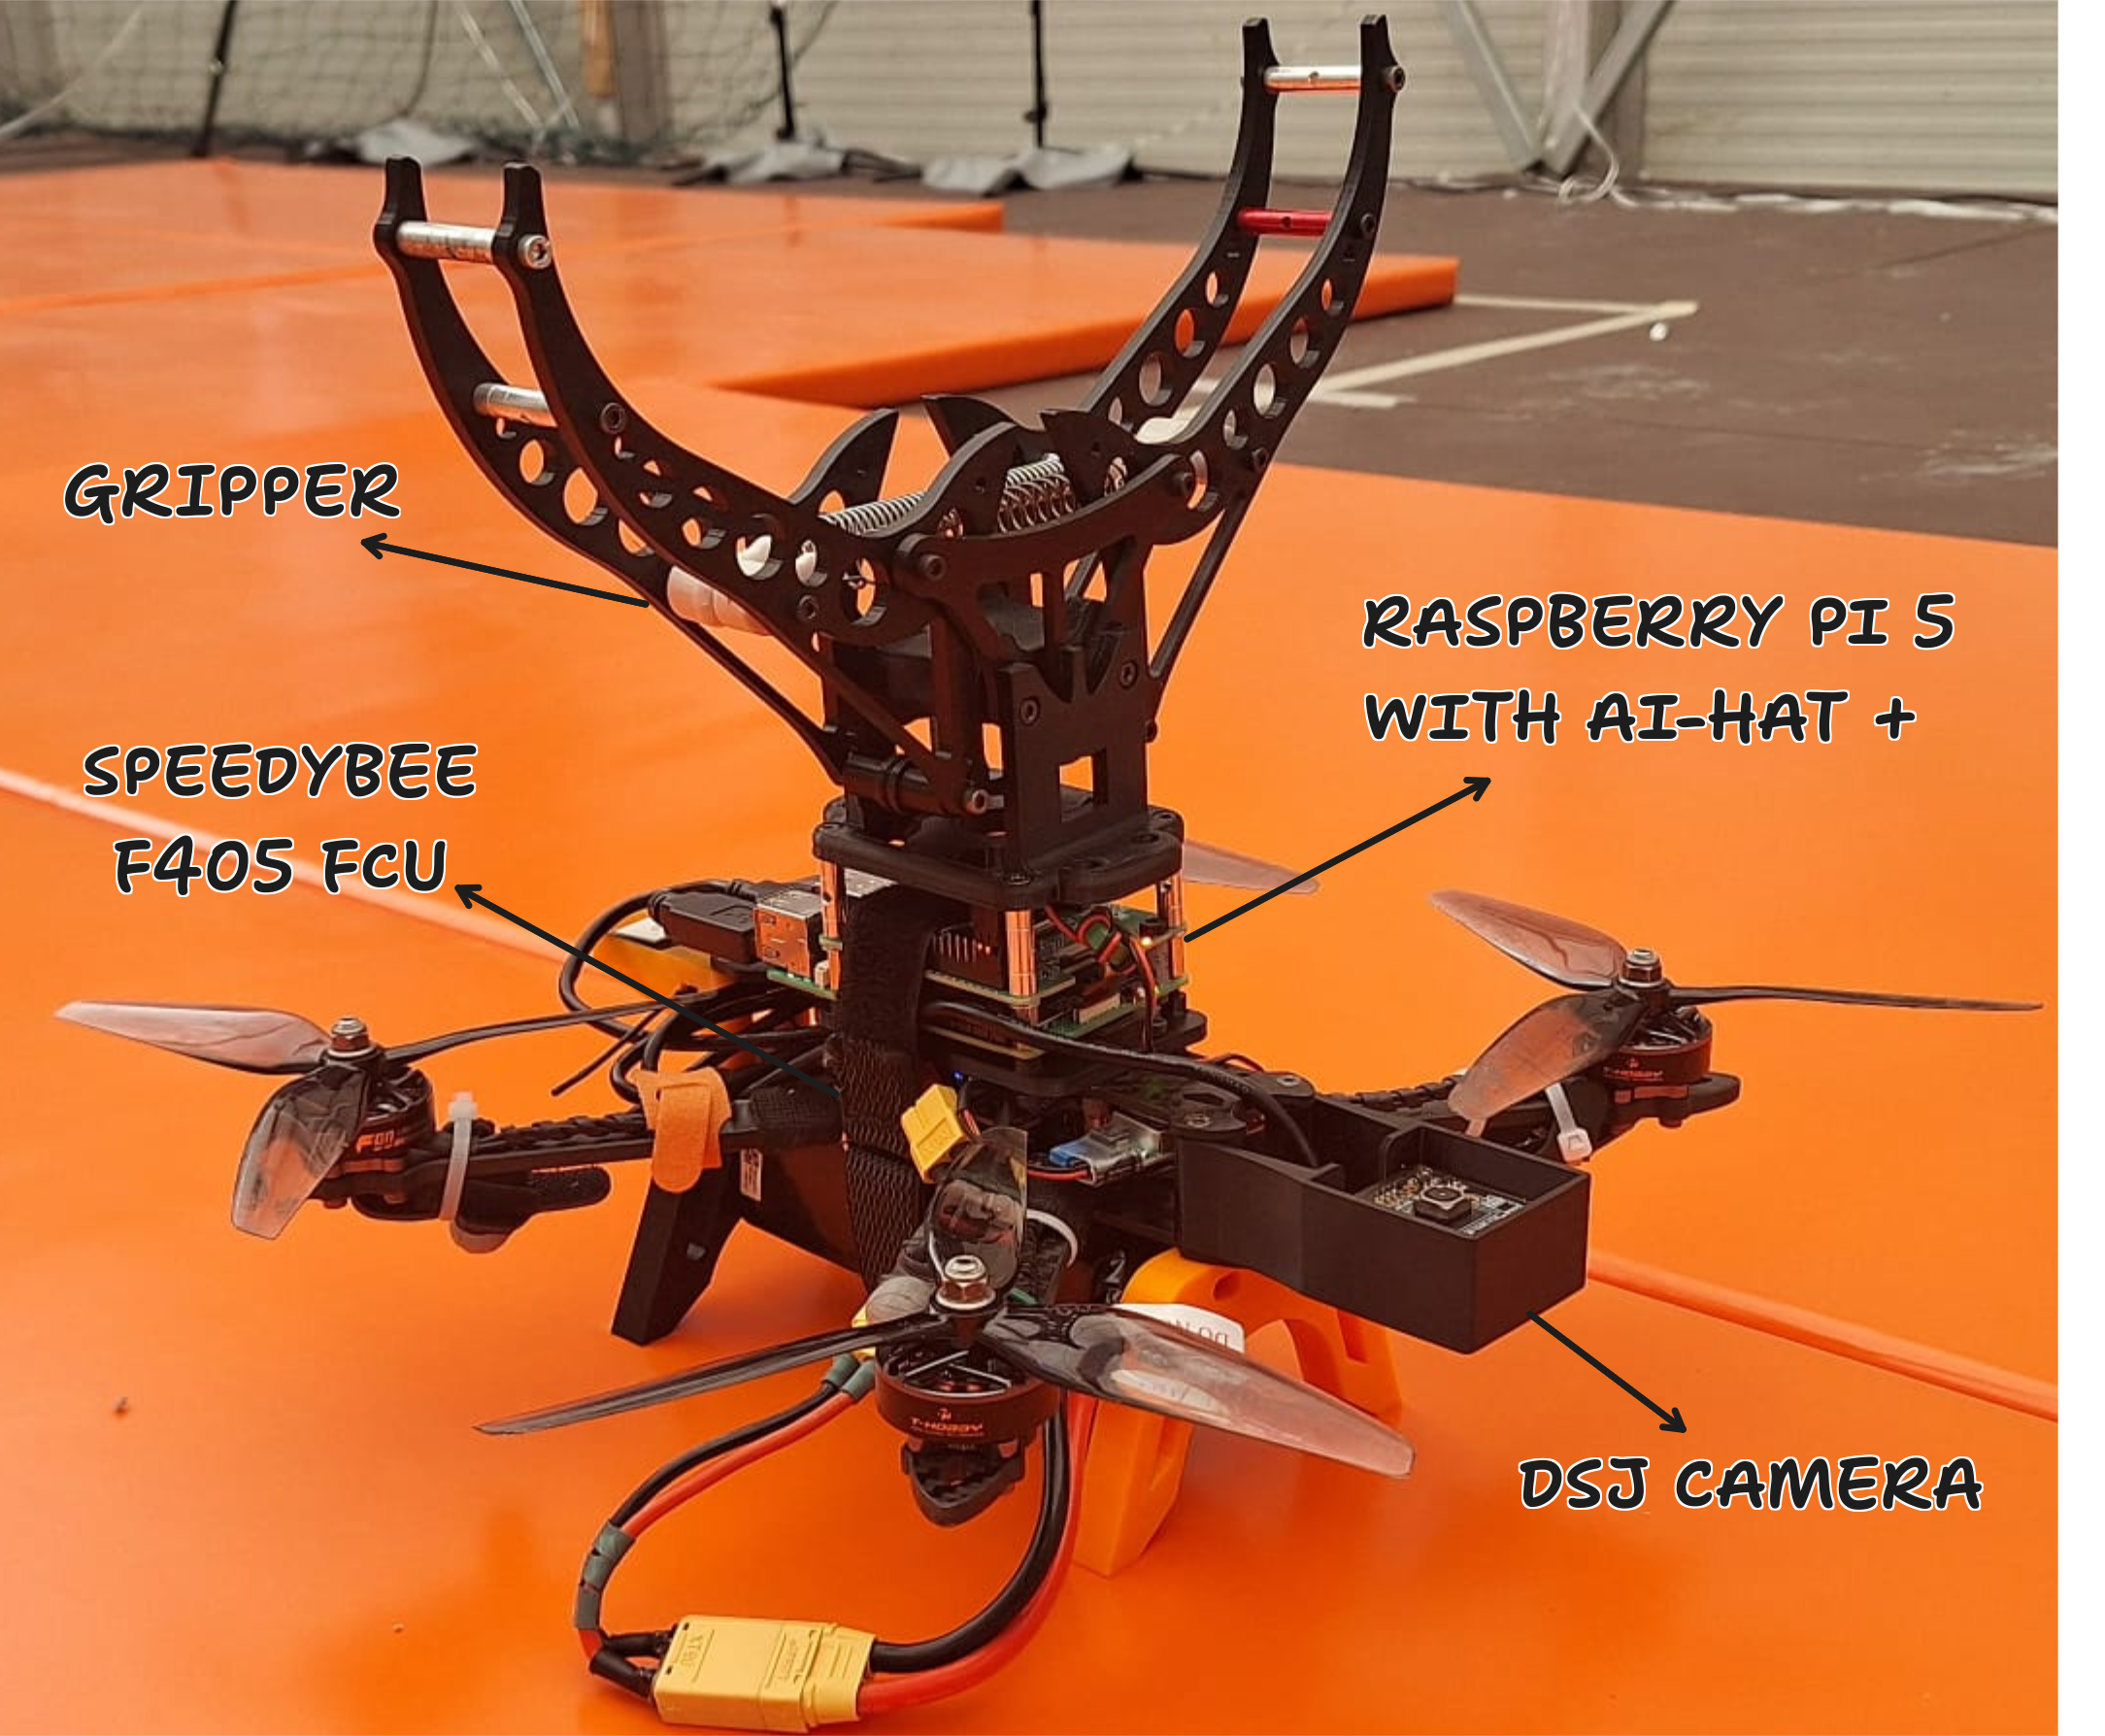
\includegraphics[width=0.85\textwidth]{images/uav_platform.png}
\caption{Letjelica korištena u eksperimentima s označenim glavnim komponentama: hvataljkom za prijanjanje, SpeedyBee F405 upravljačkom jedinicom, Raspberry Pi 5 računalom s AI Hat+ dodatkom te DSJ kamerom.}
\label{fig:uav_platform}
\end{figure}

\subsection{Računalo i senzori na letjelici}
Računalo na letjelici je Raspberry Pi 5 s 8 GB radne memorije, uz Raspberry Pi AI Hat+ dodatak s Hailo-8 akceleratorom (28 TOPS) za sklopovski ubrzano zaključivanje modela. Kao izvor slike koristi se DSJ-3079-HE, standardna USB (UVC) kamera spojena preko V4L2/OpenCV sučelja bez potrebe za posebnim upravljačkim programom, snima pri rezoluciji 1280×720 piksela i 30 sličica u sekundi.

\subsection{Mehanizam za prijanjanje}
Za prijanjanje se koristi prilagođena 3D-tiskana pasivna hvataljka s oprugom, izrađena od PETG materijala, montirana na okvir letjelice. Hvataljka ostaje otvorena dok se na unutarnji dio čeljusti ne primijeni dovoljna sila, nakon čega se hvataljka zatvara.

\section{Arhitektura sustava}
\label{sec:arhitektura}

% TODO: umetnuti dijagram arhitekture sustava

Sustav je podijeljen na dva izvedbena okruženja koja se izvode na istom fizičkom računalu (Raspberry Pi 5), ali u odvojenim programskim okolinama: Raspberry Pi OS, na kojem se izvodi percepcijski cjevovod, i Ubuntu unutar Docker kontejnera, na kojem se izvodi ROS upravljački sloj. Ta se podjela zadržava jer AI Hat+ akcelerator komunicira isključivo s Raspberry Pi OS okruženjem, pa sve što ovisi o slikovnim podacima i modelima dubokog učenja ostaje na toj strani.

Percepcijski cjevovod (poglavlje~\ref{ch:percepcija}) na ulazu preuzima okvire s kamere, a na izlazu proizvodi jednu pikselnu točku prijanjanja u slikovnoj ravnini. Ta se točka šalje preko UDP-a u Docker okruženje, gdje je preuzima upravljački sloj (poglavlje~\ref{ch:upravljanje}) koji je preslikava u naredbe kutne brzine tijela i brzine penjanja za letjelicu. Sučelje između dviju strana sustava jest jednostavna poruka koja nosi pikselnu poziciju ciljne točke u slici (\texttt{point\_x}, \texttt{point\_y}), čime se zadržava jasna granica između percepcije (koja ne zna ništa o geometriji letjelice ni o načinu upravljanja) i upravljanja (koje ne zna ništa o tome kako je točka detektirana ni kojim je modelom dobivena).

Izbor UDP-a kao poveznice između dviju strana sustava posljedica je same podjele na odvojena izvedbena okruženja: Raspberry Pi OS i Docker kontejner ne dijele isti procesni prostor, pa izravno dijeljenje memorije ili poziv funkcija nije moguć, a jedina veza između njih jest mrežno sučelje. Budući da se prenosi samo jedna točka po sličici, bez potrebe za jamstvom isporuke ili redoslijeda, UDP je dovoljan i jednostavniji od uspostave punog ROS mosta ili TCP veze između okruženja.

Percepcijska i upravljačka strana sustava rade na različitim, međusobno neusklađenim taktovima. Izlazna frekvencija modela detekcije nije fiksna: ovisi o vrsti detekcije i broju grana prisutnih u kadru, a kod stvarne detekcije grana na Raspberry Pi 5 pada na oko 4,6 Hz unatoč tome što kamera isporučuje 30 sličica u sekundi (vidi Odjeljak~\ref{sec:treniranje-modela}). Upravljački sloj \texttt{ibvs\_perching} naredbe objavljuje znatno češće, pri 30 Hz, pa bi izravno oslanjanje na izlaz modela detekcije u svakoj iteraciji upravljačke petlje predstavljalo usko grlo. Taj se problem rješava KLT praćenjem: nakon zaključavanja točke prijanjanja, model detekcije prestaje raditi, a značajke izdvojene iz referentne slike prate se optičkim tokom znatno većom frekvencijom, čime upravljački sloj u svakoj iteraciji prima ažuriranu procjenu položaja cilja, a ne zastarjelu vrijednost iz posljednjeg pokretanja modela. Detaljan opis ovog mehanizma dan je u Odjeljku~\ref{subsec:klt}.

Ovakva podjela odgovornosti nije samo posljedica sklopovskog ograničenja (Hailo-8 akcelerator dostupan isključivo na strani Raspberry Pi OS-a), nego i namjeran dizajnerski izbor koji dopušta zamjenu percepcijske strane bez izmjene upravljačkog sloja. To je u ovom radu i iskorišteno: isti upravljački sloj korišten je i s ArUco modulom za detekciju oznaka (poglavlje~\ref{ch:eksperimenti}) i s cjevovodom za detekciju grane, budući da oba proizvode identično sučelje prema Docker strani.
